\part{Vers une synergie homme-machine}
    Alors que l'intelligence artificelle a un penchant "buzzword" utilisé par des entreprises pour 
    mieux vendre leur produit en faisant l'association IA égal à plus de performances, et que les 
    site et média d'informations montre du doigt l'intelligence artificelle comme le futur destructeur 
    d'emploi, il est important de souligner que les êtres humains sont passé par de telles phases 
    auparavant: \newline 

    \begin{itemize}
        \item La révolution agricole:En Europe, pendant le 18ième siècle moins de terres en jachère,
        << En 1840, 7 millions d'hectares c'est-à-dire 25\% 
        des terres européennes sont en jachère ; en 1900, il n'y a plus que 3
         millions d'hectares en jachère, c'est-à-dire 10 \% des terres. >>
         \footnote{source: \url{https://www.philisto.fr/cours-49-transformations-economiques-de-l-europe-xixe-siecle.html}}
         l'apparition de la moissonneuse et la batteuse à vapeur changent les méthodes agricoles 
         vers une agriculture orienté capitalisme. 
         Cette transformation a été globalement avantageuse pour tout le peuple, l'utilisation 
         des machines étant rare à cause de leur prix, l'utilisation d'animaux de traits ne 
         disparaitra que très progressivement ne laissant pas sans capacité de travail les personnes
         qui dépendaient de leur utilisation dans l'agriculture (la mecanisation ne s'effectuera 
         massivement qu'a partir de la fin de la seconde guerre mondiale). \newline 

         \item La révolution industrielle: c'est la transformation qui aura eu le plus grand impact,
         elle est decomposé en deux temp qui peuvent globalement être associé avec 
         l'utilisation de la machine à vapeur puis l'apparition de l'electricité, du gaz ainsi que 
         moteur à explosion, l'exode rural qui s'ensuit (fuir la campagne et son agriculture pour 
         rejoindre la ville et ses usines) et dû à une jeunesse formé à l'agriculture 
         qui ne voyait pas de futur dans l'agriculture et une opportunité dans l'industrie. \newline
    \end{itemize}

    cette période montre que l'homme et les nations ont les capacités pour s'adapter 
    aux paysages économiques en perpétuels changement, mais les challenges à surmonter 
    avec l'intelligence artificelle sont différents puisqu'elle va et a déjà bousculée tout 
    les domaines y compris l'agriculture et l'industrie, malgré cela pour que cette 
    révolution soit aussi disruptives il y a de nombreux challenges à dépasser.


    \chapter{Surmonter les problèmes inhérent au machine learning }
        Des problèmes empecheront l'intelligence artificelle notamment à cause de l'utilisation 
        du machine learning, technologie qui va rester d'actualité pendant de nombreuses années car nous
        avons qu'effleuré la surface et les possibilités de celle-ci.
        Tout d'abord le principe d'explicabilité, la difficulté de reproductibilité et enfin l'applicabilité 
        métiers sont les trois principaux points bloquants pour une évolution positive de 
        l'intelligence artificielle. \newline

        \section{Explicabilité et interprétabilité}
            \subsection*{Définitions}
            Explicabilité: 
            \begin{quote}
                << Une décision algorithmique est dite explicable s’il est possible d’en rendre compte 
                explicitement à partir de données et caractéristiques connues de la situation. 
                Autrement dit, s’il est possible de mettre en relation les valeurs prises 
                par certaines variables (les caractéristiques) et leurs conséquences  
                sur la prévision, par exemple d’un score, et ainsi sur la décision. >>
                \footnote{Source: \url{https://perso.math.univ-toulouse.fr/mllaw/home/statisticien/explicabilite-des-decisions-algorithmiques/}}
                \newline 
            \end{quote}

            Interprétabilité:
            \begin{quote}
                << Une décision algorithmique est dite interprétable s’il est possible d’identifier 
                les caractéristiques ou variables qui participent le plus à la décision, 
                voire même d’en quantifier l’importance. >>
                \footnote{Source:\url{https://perso.math.univ-toulouse.fr/mllaw/home/statisticien/explicabilite-des-decisions-algorithmiques/}}
                \newline
            \end{quote}

            Une des raison de la resistance au changement est l'incapacité à comprendre 
            le fonctionnement interne d'une intelligence artificelle utilisant le machine learning, 
            ce qui rend une entreprise dépendant de cette dernière avec un maîtrise relative
            entre les mains des data scientists. \newline

            Prenon l'exemple d'un algorithme standard, par exemple un arbre syntaxique abstrait
            dans compilateur, il est aisé de comprendre le fonctionnement de chaque partie 
            de l'arbre et l'impact dans le cas du changement de la valeur d'un noeud.
            Dans le cas d'un algorithme de reconnaissance d'image par machine learning 
            il est bien plus difficile de comprendre les variables en jeux lors du changement 
            d'un pixel par exemple, aujourd'hui l'explicabilité et l'interprétabilité
            du deep learning est nulle. \newline

            \begin{figure}[H]
                \centering
                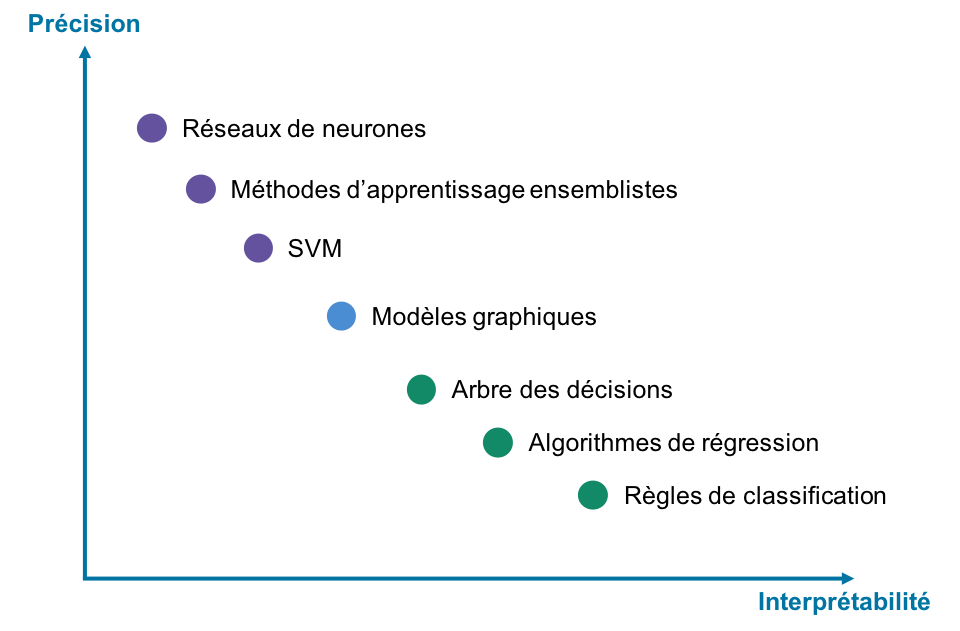
\includegraphics[width=0.7\textwidth]{Images/accvsint}
                \caption{Précision vs Interprétabilité - actuia.com}
                \label{fig:explicability}
            \end{figure}

            En réalité plus un algorithme de machine learning est précis et fiable 
            plus sont interprétabilité devient faible, le système <<deviens une boite 
            noire>>, malheureusement par défaut les réseaux de neurones semblent 
            être dans le bas du panier. \newline 
            
            Une intelligence artificelle en capacité de répondre aux besoins d'explicabilité 
            doit pouvoir répondre aux questions suivantes: \newline 

            \begin{itemize}
                \item Objectif d'une opération
            \end{itemize}

            
            \begin{figure}[H]
                \centering
                
\includegraphics[width=0.7\textwidth]{Images/explicabilite}
                \caption{Enjeux de l'explicabilité - actuia.com}
                \label{fig:explicability}
            \end{figure}



        \section{Reproductibilité}
        L'explicabilité permettrait de faciliter la reproductibilité, tandis que sans celle-ci 
        aujourd'hui les data scientists rencontre une difficulté majeur: 
        l'incapacité à reproduire les modèles de machine learning d'autres data scientists 
        et chercheur voir même l'incapacité à reproduire ses propres modèles. \newline 
            



        \section{Applicatibilité Métier}
            Cette problématique concerne l'identification des besoins auquels l'intelligence artificelle 
            peut répondre, comme indiqué dans la partie précèdente une des principales difficulté réside 
            dans l'application concrète de celle-ci, à quel(s) besoin(s) peut répondre une 
            intelligence artificelle qu'un algorithme "traditionnel" ne peut pas ? 



        %utilisation humain va shifter dans le luxe et petites serie dans l'industrie 
        %un peu comme les voitures  monté à la main 
        %un effet d'elite 
        %l'IA va devenir le "bas de gamme" de la création de bien 
        %tandis que les industries et à echelle humaine vont rentrer dans le luxe ? 
        %le luxe ne "subis pas la crise"

        %services utilisant l'IA pour desservir les endroit qui on peu ou pas accès 
        %à lesdit services (ex: campagne )
    \chapter{Automatiser les taches sans grande valeur ajoutée}

        Nous avons vous dans la partie précédente que l'intelligence artificelle
        ne pourra pas remplacer l'intelligence artificelle dans tout 
        les domaines qui demande de la créativité, de l'empathie et globalement 
        la majorité des domaines qui demande des intéractions complexes entre 
        individus tel que la gestion de projet, l'analyse du besoin et la 
        diplomatie. Il faut donc étudier quels métiers peuvent être automatisés dans le futur proche,
        voici une classification des caractéristiques d'un métier qui peut être automatisé:
        \newline
        \begin{itemize}
            \item Taches simples et répétitives, répétition basique mais non absolue, des automates 
            comme dans les industrie automobiles peuvent remplir le rôle, on parle ici de tâche 
            répétitive mais non deterministes.
            \newline

            \item Communication simple avec un être humain tel que le démarchage téléphonique,
            gestion de demande administrative (statut d'un dossier, demande de document), 
            la reception / accueil où la gestion d'appel et d'agenda peut facilement être automatisé,
            le domaine comptable dans lequel il y a dèjà des offres qui automatise fortement 
            la comptabilité tel que QuickBooks et FreshBooks.
            \newline

            \item Taches simples non répétitives comme 
            les voitures taxi, les véhicules de livraison, l'objectif est d'aller d'un point A à 
            un point B. \newline
        \end{itemize}
        
        
        %bonne idée ou pas ?
        \section{La valeur intrinsèque de métiers qui ne semblent pas en avoir }
        \section{Re-spécialisiation au sein des métiers automatisés}

        %exemple des banquiers avant les distributeurs automatique qui se sont respecialisé 
        %dans le conseil client et le commercial
        %la proposition d'offre, la gestion d'investissement
        
        %explicabilité des IA: les IA qui détail leur "reflexion" pour arriver à leur résultat 
        % => moins de resistance au changement 
        %as automation frees our time it increases the scope of what is possible we invent new ideas
        %new products
        %O-ring principle
        %automation: create more wealth in less time
        %build society with opportunity, problems is the institution
        % 

    \chapter{Utiliser l'IA comme un assistant de productivité}
